\section{Outreach}

As a team, de.evolution believes that robotics is more than just the engineering. Our first year as a team we saw that the other FTC team at our school, Domo Arigato, was entirely seniors and we were sad that it was going to disappear. This inspired us to try and spread robotics to the younger students and have people involved to keep robotics teams going and to propogate the message of FIRST throughout our community. We have started a robotics class at our high school which has turned into the team Domo Arigato. Due to the popularity of the class a second class, and subsequently an FTC team, has been started. Both the Robo Ravens and Domo Arigato, along with our own team, de.evolution, work hard to start a robotics and engineering culture at our school. The section will be structured as follows, we will begin by listing our community outreach and will in the subsequent subsections go into further detail about some of the more important work we do

\subsection{Community Outreach}
As a team, de.evolution has tried to do a lot to help spread the ideas of FIRST, robotics and engineering. The following is an extensive list of some of the community outreach that we have done:

\begin{enumerate}
	\item Robotics demos to elementary school students at Solana Pacific Elementary, Del Mar Heights Elementary, Rancho Santa Fe Elementary
	\item PTC World demo in June 2013
	\item Mentoring of the three Islamic School of San Diego FLL teams 
	\item Sister team of the San Dieguito Academy FTC teams Paradox Squared and Paradox Cubed
	\item Demo for school board \& superintendent – sponsored building/engineering production district-wide with bond measure
	\item Hosted Robotics Week at CCA in coordination with Domo Arigato (3513)
	\item Publication in newspapers \& press releases about STEM/robotics
	\item Publication in school's magazines
	\item Over 20\% of school has become involved with the FIRST robotics programs after the inception of our team
	\item Inspired the FIRST robotics classes
	\item Incorporating art and conservatory at CCA with the robotics program
	\item Incorporating the humanities conservatory at CCA with the robotics teams
	\item Working with TEDxYouth@SanDiego to spread robotics to the students in San Diego
	\item Attended and presented at Rotary meetings to show our community the influence of robotics
\end{enumerate}

\subsection{In-person demos at middle and elementary schools}

We have presented the FIRST Tech Challenge to three separate elementary schools: Solana Pacific Elementary, Del Mar Heights Elementary, and Rancho Santa Fe Elementary. We inspired the creation of teams at these schools this FTC season, and will bring them into our robotics program at Canyon Crest Academy if they choose to attend our school.

\begin{fancyquotes}
Ever since last spring, when their team members did a presentation at our school for Science Discovery Day, they have been an inspiration to our robotics students and are chiefly responsible for encouraging our 8th graders to start an FTC team this year. \newline \newline
--David Warner, Coach for the RSF Eagles FTC Team
\end{fancyquotes}

When we showed our robot to the students at these schools we had their teachers drive the robot. The kids loved it! It was definitely a great experience for us to be able to show so many students how much we loved robotics and the subtle beauty that is found in engineering and FIRST competitions. 

The students at the schools are interested in robotics, and are now aware of what the FIRST program can provide. We are thrilled to have the opportunity to interest more students in FTC, and look to continue doing so next year!

\subsection{Helping other teams online}
As the majority of the members on our team are also on the FRC team \underline{The Aluminum Narwhals} we realize that having online support is one of the best ways to debug and learn about robotics. Chief Delphi, one of the prominent places for online FIRST discussion, is very popular among FRC teams. However, FTC teams do not have nearly as much online support as they may need or like. As a team we have shifted a lot of our focus to helping teams online. We have open-sourced all of our code and have created code tutorials to help out many other teams. We have helped teams in the following ways

\subsubsection{Syntax Error code optimization assistance}

At a San Diego regional qualification competition, we entered a discussion with team 6077, Syntax Error, about code optimization. We were sharing our varied tricks which were used in code, and through discussion, it became clear that there were a couple points they were particularly interested in implementing. We passed them some contact information, and later received an email from them:

\begin{fancyquotes}
Hey Noah,

We're interested in optimizing the speed of our teleop code, and I know you had mentioned at the tournament that you guys XOR-ed the joystick values to determine when the values had changed--allowing you to skip checks when things weren't changing. Could you please go into more depth as to how you achieved this? Did you directly modify joystickdriver.c? Which values should we be XOR-ing exactly?

Thanks,

-Collin 
\end{fancyquotes}

We wrote out a document generally detailing the approaches we took when optimizing our teleoperated code. My response was the following PDF file:

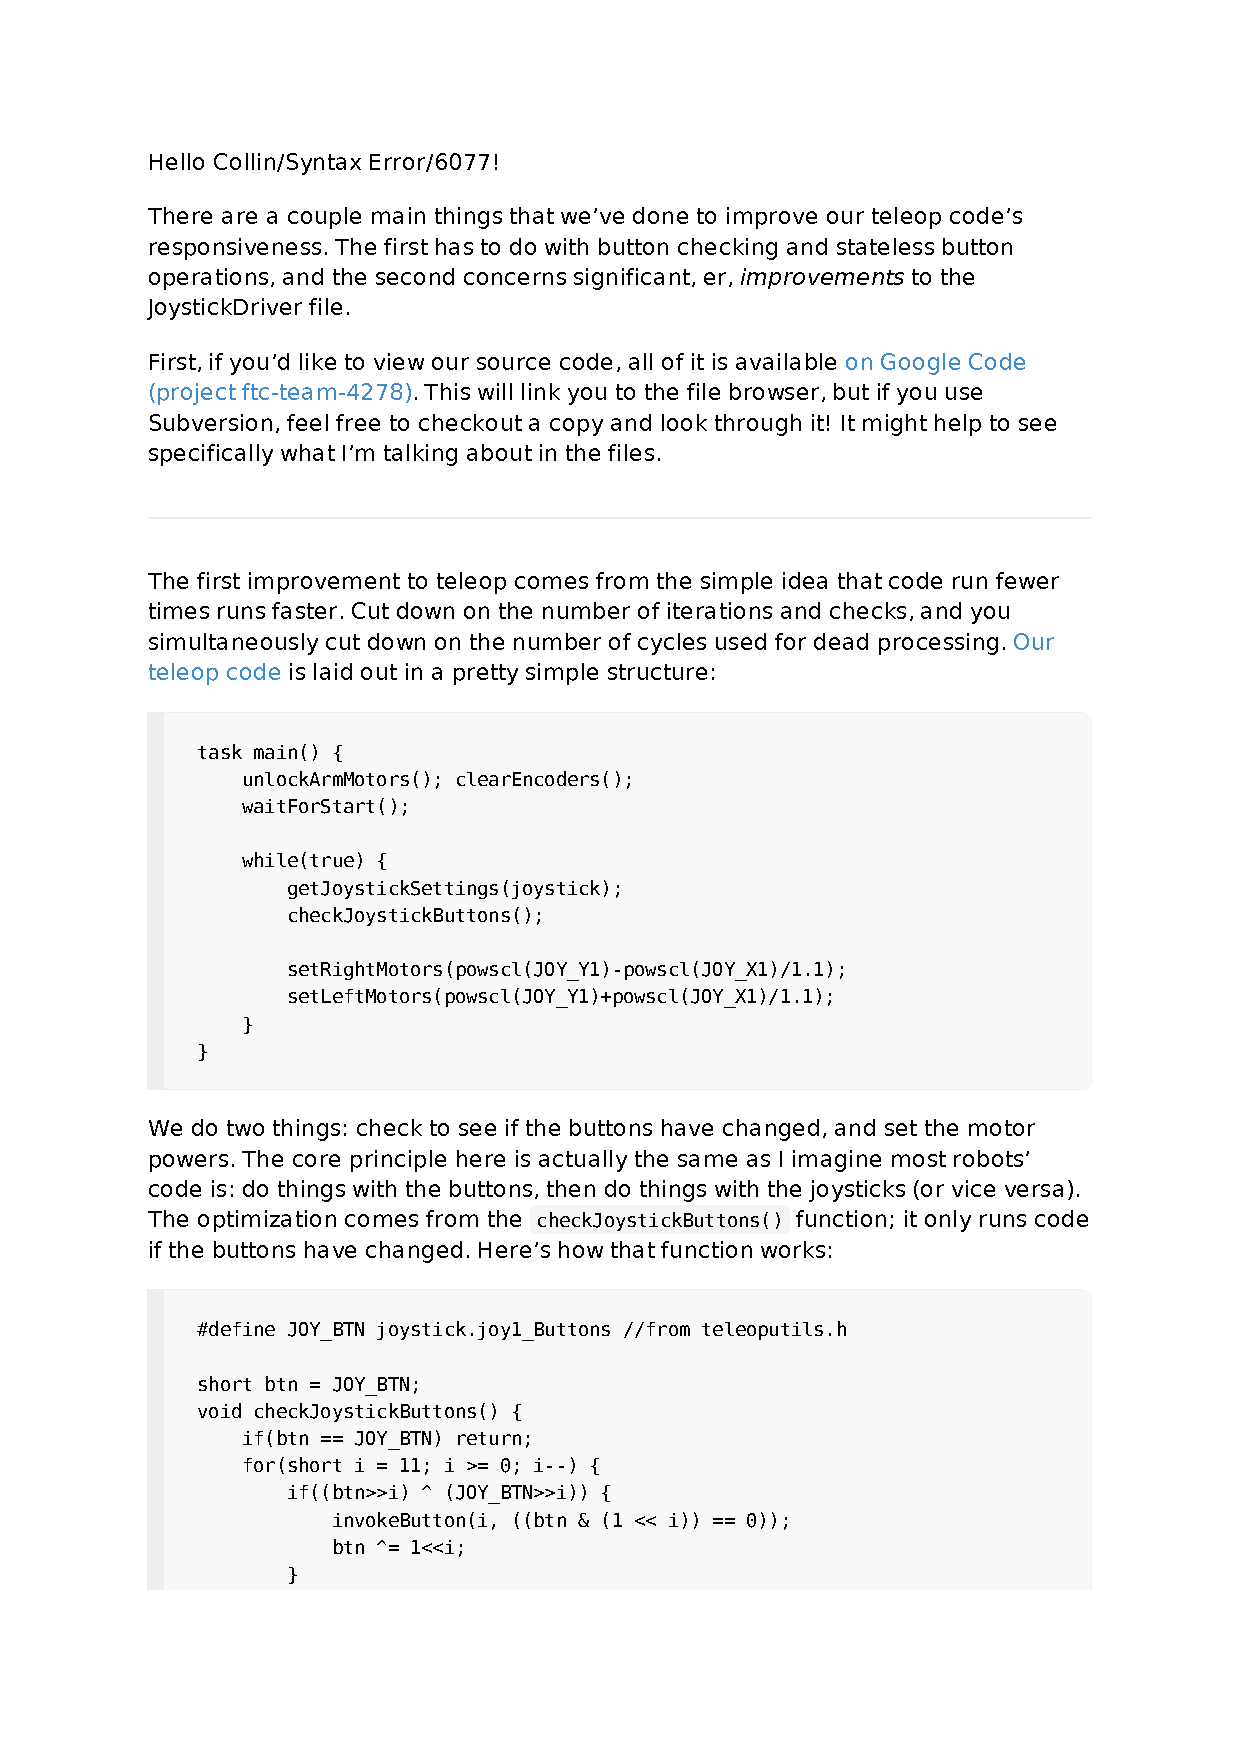
\includepdf[pages={1-2}]{SyntaxError.pdf}

The aim was to create an easy-to-follow guide for someone with experience to optimize the teleoperated program. To our enjoyment, they reported significant increases in response time on their controller.

\subsubsection{Reddit}
To our pleasant surprise the FTC Reddit subforum was started this year and our team has jumped completely on board to help other teams with both programming and mechanical help. We often will have Skype calls with other teams around the country or just send long documents to them. We have also created extensive and comprehensive documents that detail all of the details, including the advantages and disadvantages, of the different drive trains. The following pages have some of our biggest discussions with teams on Reddit:

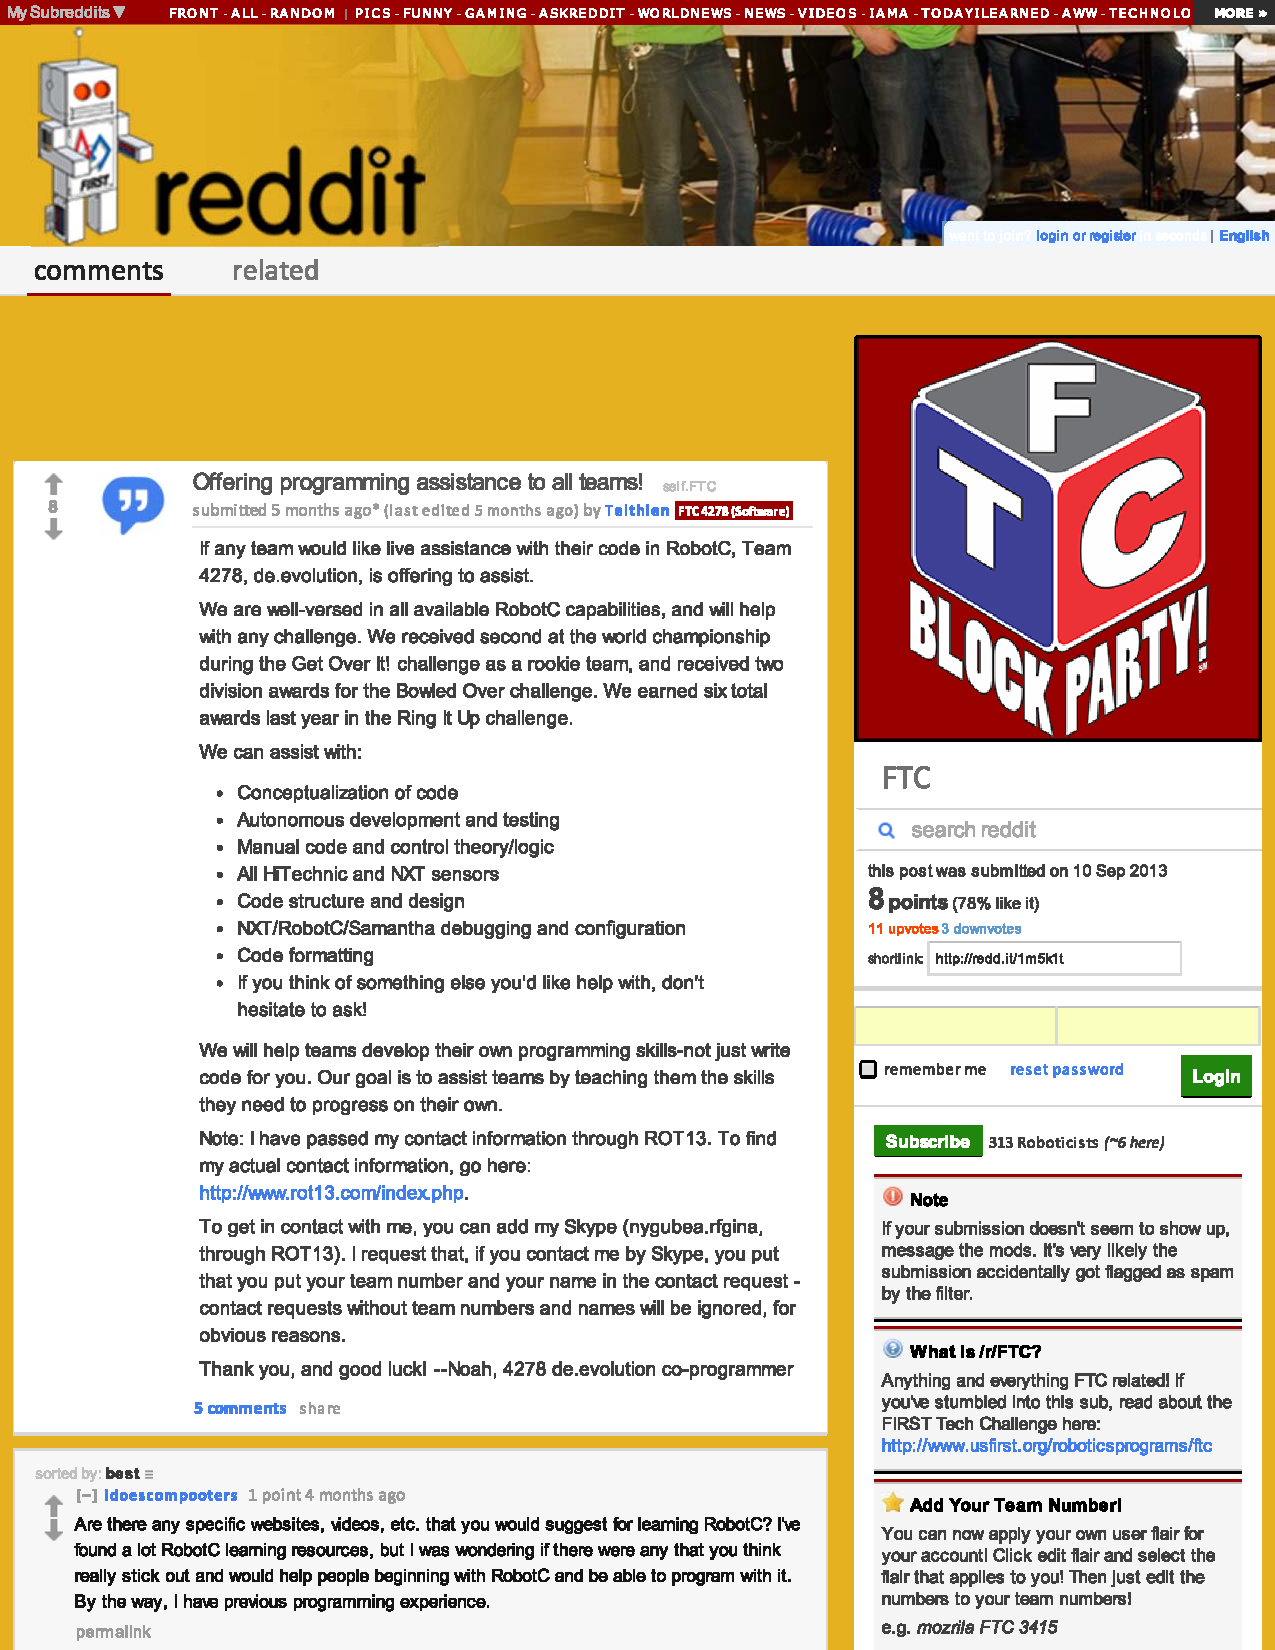
\includepdf[pages={-}]{CodeHelp.pdf}
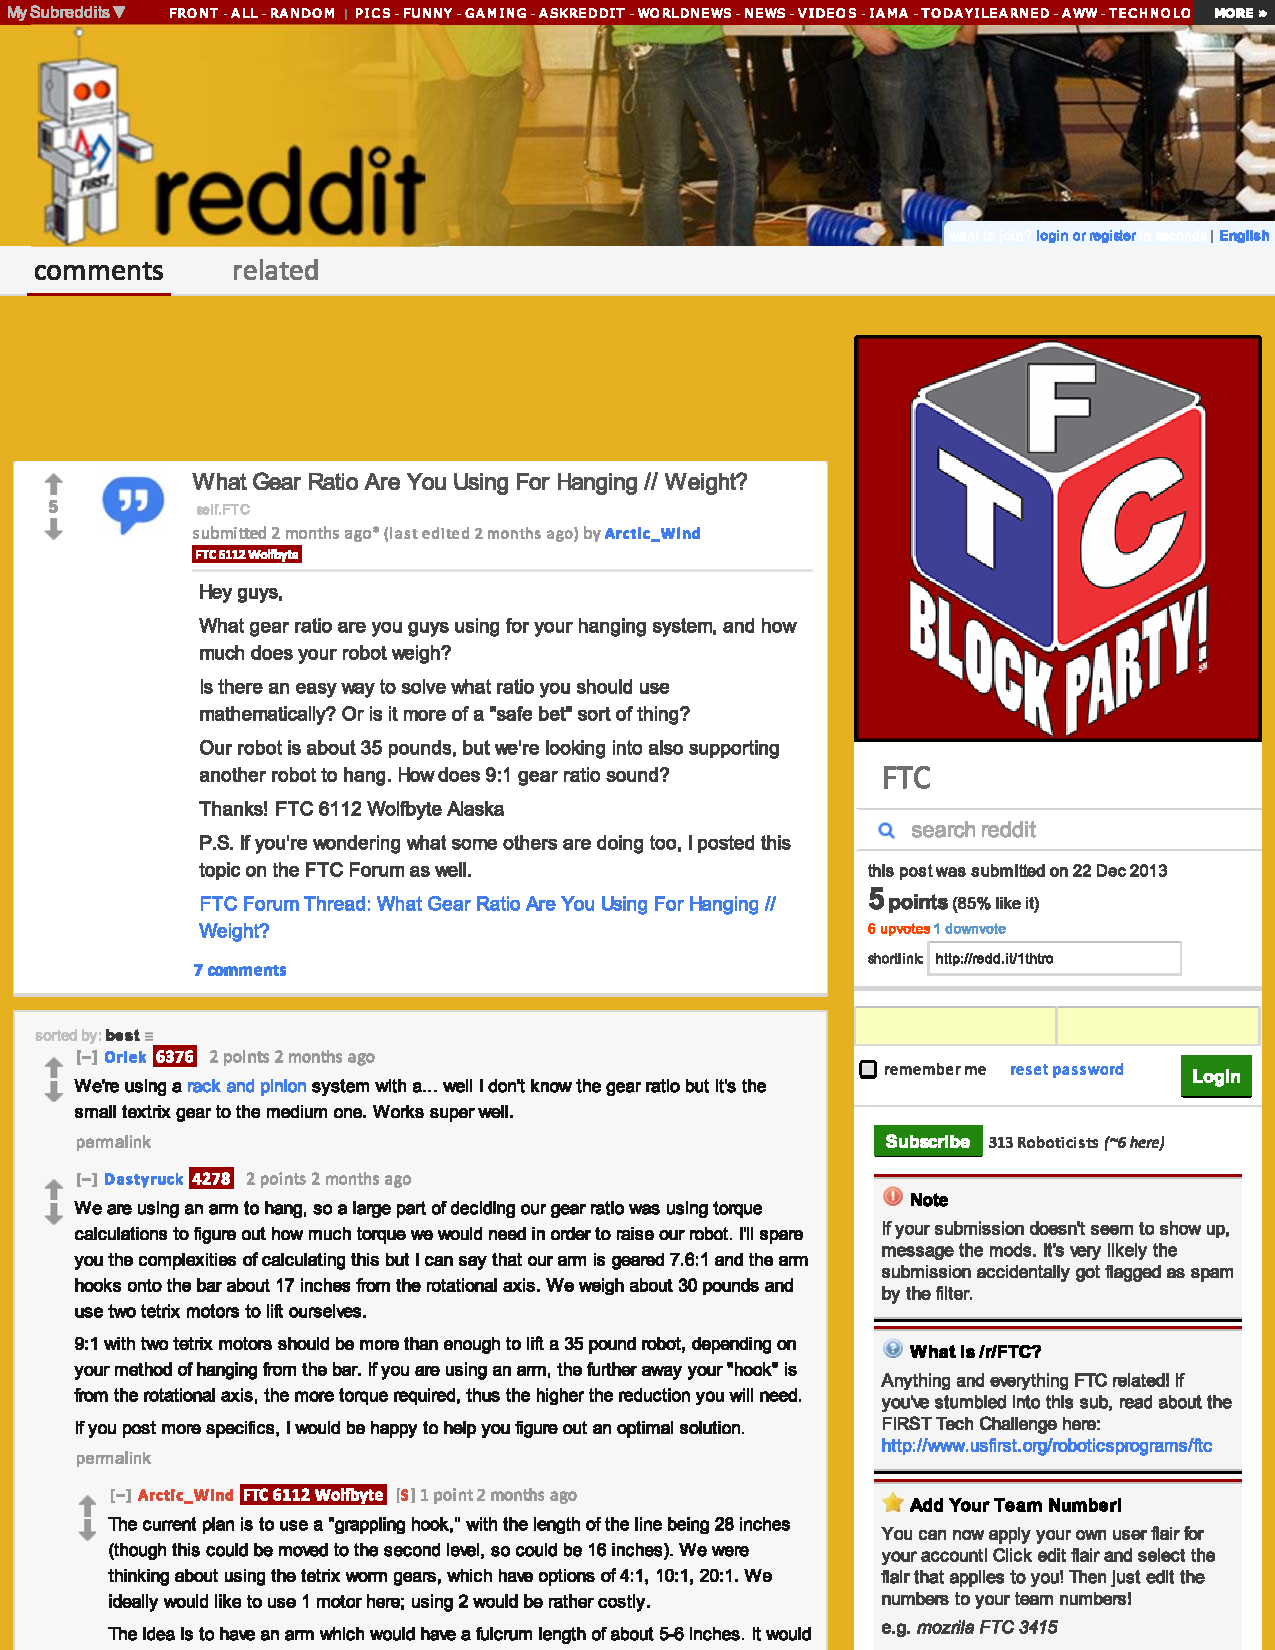
\includepdf[pages={-}]{FTCHanging.pdf}
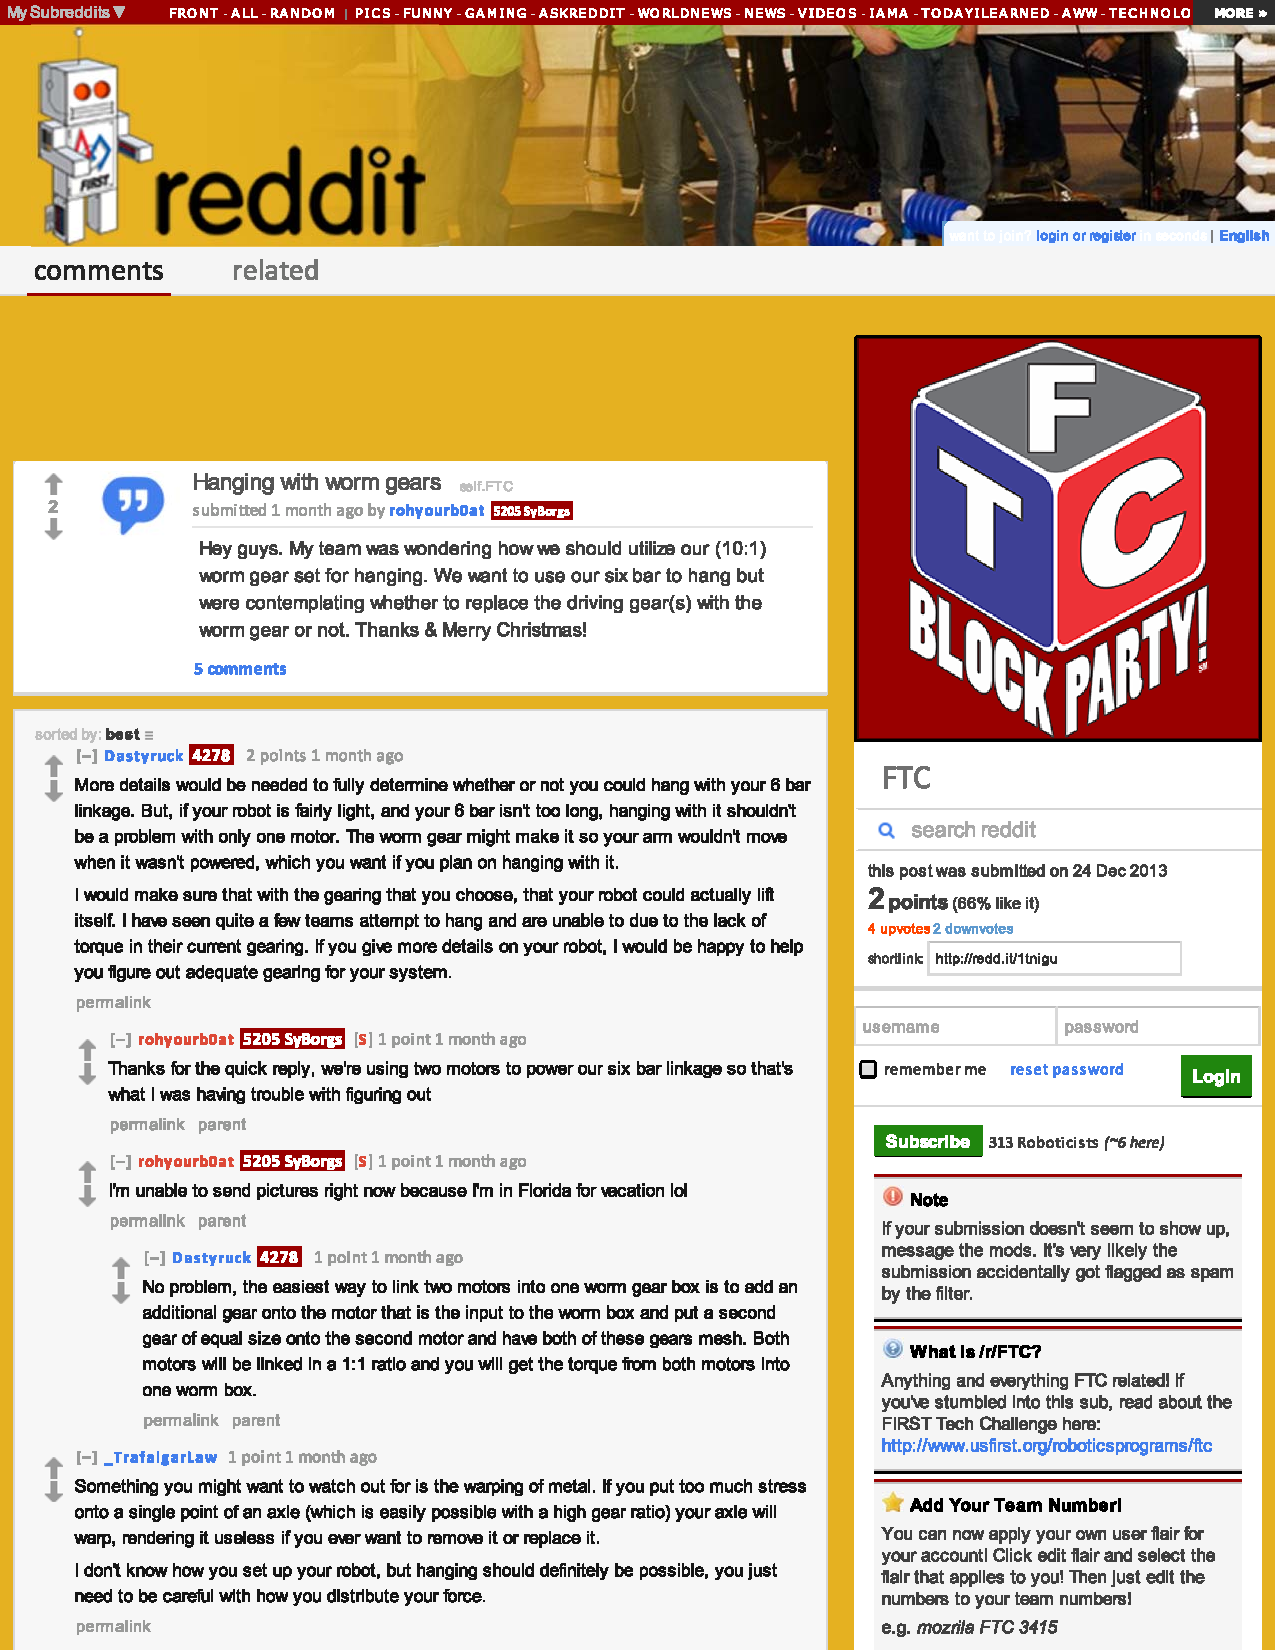
\includepdf[pages={-}]{GearingFTC.pdf}

Additionally, the code assistance post was also mirrored on the Chief Delphi FRC forums. We have contacted six teams through these mediums. 

\subsubsection{FTC Team NESI (6033)}

One of the many responses we received for our online posts has been copied here. In short: a team was in need of holonomic drive assistance, and we responded with details about how the algorithm might best be implemented. We did so with the intent to provide a conceptual structure, while still leaving an educational problem for the team to understand and develop. In this way, we are not simply giving them the solution; we are instead helping them understand the tools they need to implement a solution, furthering their understanding and education.

\begin{fancyquotes}
I saw your offer to help teams with programming. We are a new FTC all girls team and could use some help with programming our robot. We originally had tank drive and were able to modify the code to work. However, we thought omni direction would be be better for us and built a [chassis] with omni directional wheels mounted at 45 degrees in each corner with a motor on each. There is an encoder on each. I know there has to be some conversion to establish drive vectors, but having some challenges with that. If you had some sample RobotC code that would be great. The girls are very sharp and could make it work, we just need a little help. Ideally we want to use one joystick to go forward, back, left, right. Then the other joystick to rotate left or rotate right.
 
Anything you can do to provide sample code would be VERY much appreciated! Thanks!

\textit{Coach Jerry, Team NESI (6033)}
\end{fancyquotes}

Our approach to helping teams in this situation is not to outright give the solution, but help provide a conceptual framework for thinking about approaching a solution. That way, teams still gain the educational experience of solving problems themselves, but aren't working in the dark when they attempt to solve the problem.

\begin{fancyquotes}
I'd be happy to explain conceptually! I'm sure you and I would both agree that, even though I could simply give source code, it's better for the programmers to come up with it themselves to gain a conceptual understanding. Of course, holonomic drive (45 degree omni) is confusing, so feel free to ask questions!

First, the programmers will need to have an understanding of polar coordinates. Nothing too deep, just the basics: that they are expressed with an angle and a radius. The best holonomic drive will follow sines and cosines, so I recommend converting rectangular coordinates to polar coordinates. In this way, the theta of the joystick position becomes the direction the robot is to move in, and the ``r'' magnitude becomes the speed.

There are two parts to a holonomic drive: rotation and translation. Rotation allows the robot to turn to any bearing, and translation allows the robot to move in any direction at a time. Make sure the wheels are aligned such that, in positive power, both the left and right side motors move forward.

Rotation should be added to translation, since translation is more important and complex. Thus, the goal is to work out a translation algorithm. Remember that your controller should be stored in polar coordinates. It is helpful to plot out on paper which direction you want the motors to move for each angle; for instance, at 45 degrees, you want the front left (FL) and bottom right (BR) at 100\% power, and FR/BL at 0\% power. You can use these points to build a sine/cosine graph for each wheel. 

Once a translation algorithm has been tested and implemented, rotation is the next step. Conceptually, to rotate the robot, all the wheels need to move the same direction. Thus, you can simply add whatever your rotational value is (we use the x axis on the second joystick, but be sure to divide by 128 to get a number from -1 to 1) directly to the output from the sines and cosines.

When you add rotation, you will encounter another problem: sometimes motors will be set to 200\% power, while others are at 100\%. Yet the robot still needs to turn. The cause of this problem lies in the rotation. If the robot is going at 45 degrees, FL/BR = 100\%, FB/BL = 0\%. However, if you are rotating at full power, you'll end up with a situation where FL/BR = 200\%, FB/BL = 100\%. The robot will just drive forward. What you need to do at this point is find the maximum power, and divide all the powers by it. They will stay proportional, and you'll get the expected output.

Please let me know if you have any questions! It's certainly not a simple algorithm to think about. I've tried to give a general conceptual outline of how it works, since we'd probably both agree it's better to write the code oneself. Still, if you would like further help, feel free to ask!
\end{fancyquotes}

While we have removed most of the discussion from this text, the conversation was left with:

\begin{fancyquotes}
Your explanation will be a big help to the programmers! I anticipate they will have some questions for you about how the theory gets put into practice with RobotC. Thanks for pointing out some of the troublesome aspects of how translation and rotation come together. We will be in touch. Thanks! 
\end{fancyquotes}

\subsection{Mentoring of FLL teams}
Our team aided the Islamic School of San Diego's FLL Teams during their rookie years by mentoring the young kids on robotics and the engineering design process in general. Our students voluntarily watched over the excited and energetic children, assisted in teaching them key concepts, and created useful PowerPoint presentations that were presented to further educate the FLL teams.

In each meeting, the FLL teams was taught a concept and then given time to build something from LEGOs using their newfound knowledge. Since our de.evolution volunteers were there, the FLL leader could split the team into small groups with a mentor or leader helping each group. Another advantage of having an FTC mentor available was that the volunteer could lead the team while the leader temporarily prepared the next lesson or dealt with other essential tasks. It relieved the leader of FLL and kept everything running smoothly.

The lessons taught the eager and energetic students about what causes earthquakes and the destruction that they inflict. This understanding supported the kids in cooperatively creating ideas for a machine to aid anyone who recently experienced a devastating disaster. The mentors also educated the group about the engineering design process to assist them in efficiently building a better solution when they were ready to begin fabrication of their product.

We found that mentoring FLL teams has not only allowed us to teach the students a lot about robotics, but we gained valuable experiences by doing so.

\subsection{Meeting with the SDUHSD Disctrict Office}

A while back, we met with the San Diego Union High School District (SDUHSD) district office to present the FIRST Tech Challenge program. It was a significant demonstration, as our ultimate goal was to inspire further funding for robotics in regional high schools.

Our efforts paid off. Recently, Proposition AA, an educational bond bill, was passed in the San Diego area. This included significant funding for the construction of a robotics building at our host high school, Canyon Crest Academy. We have already brought approximately 15 to 20\% of the high school population through some form of FIRST's programs, and this will hopefully expand both the educational capacity and general awareness of FIRST among the high school students.

\subsection{TEDxYouth@SanDiego}
As our team is greatly involved with Canyon Crest Academy as an academic instition we teamed up with the FRC team at our school and began creating promotional videos to show robotics to our school. At TEDxYouth@SanDiego we were invited to put on a robotics and dance choreography. We worked with the FRC team at our school and the dance conservatory to put on a truly magnificent performance. It was the joining of exceptional engineering and amazing talent in terms of the arts. 

At TEDxYouth@SanDiego, over 500 students from high school in the San Diego region all came together to be inspired. By being honored to present our robot on the TED stage we were able to reach many students and show them the elogance of robotics. By integrating it with the arts we are really able to show the practical and artistic aspect of robotics. 

\subsection{Press Releases}
To really reach the community of professionals and the general public, we turned towards press releases. By having the media come to us to cover not only our successes as a team, but our ability to inspire and reach out to many other students has given us many new opportunities to go to middle schools and mentor other FTC and FLL teams. The following pages are excerpts of some of the media and press that has covered our team:

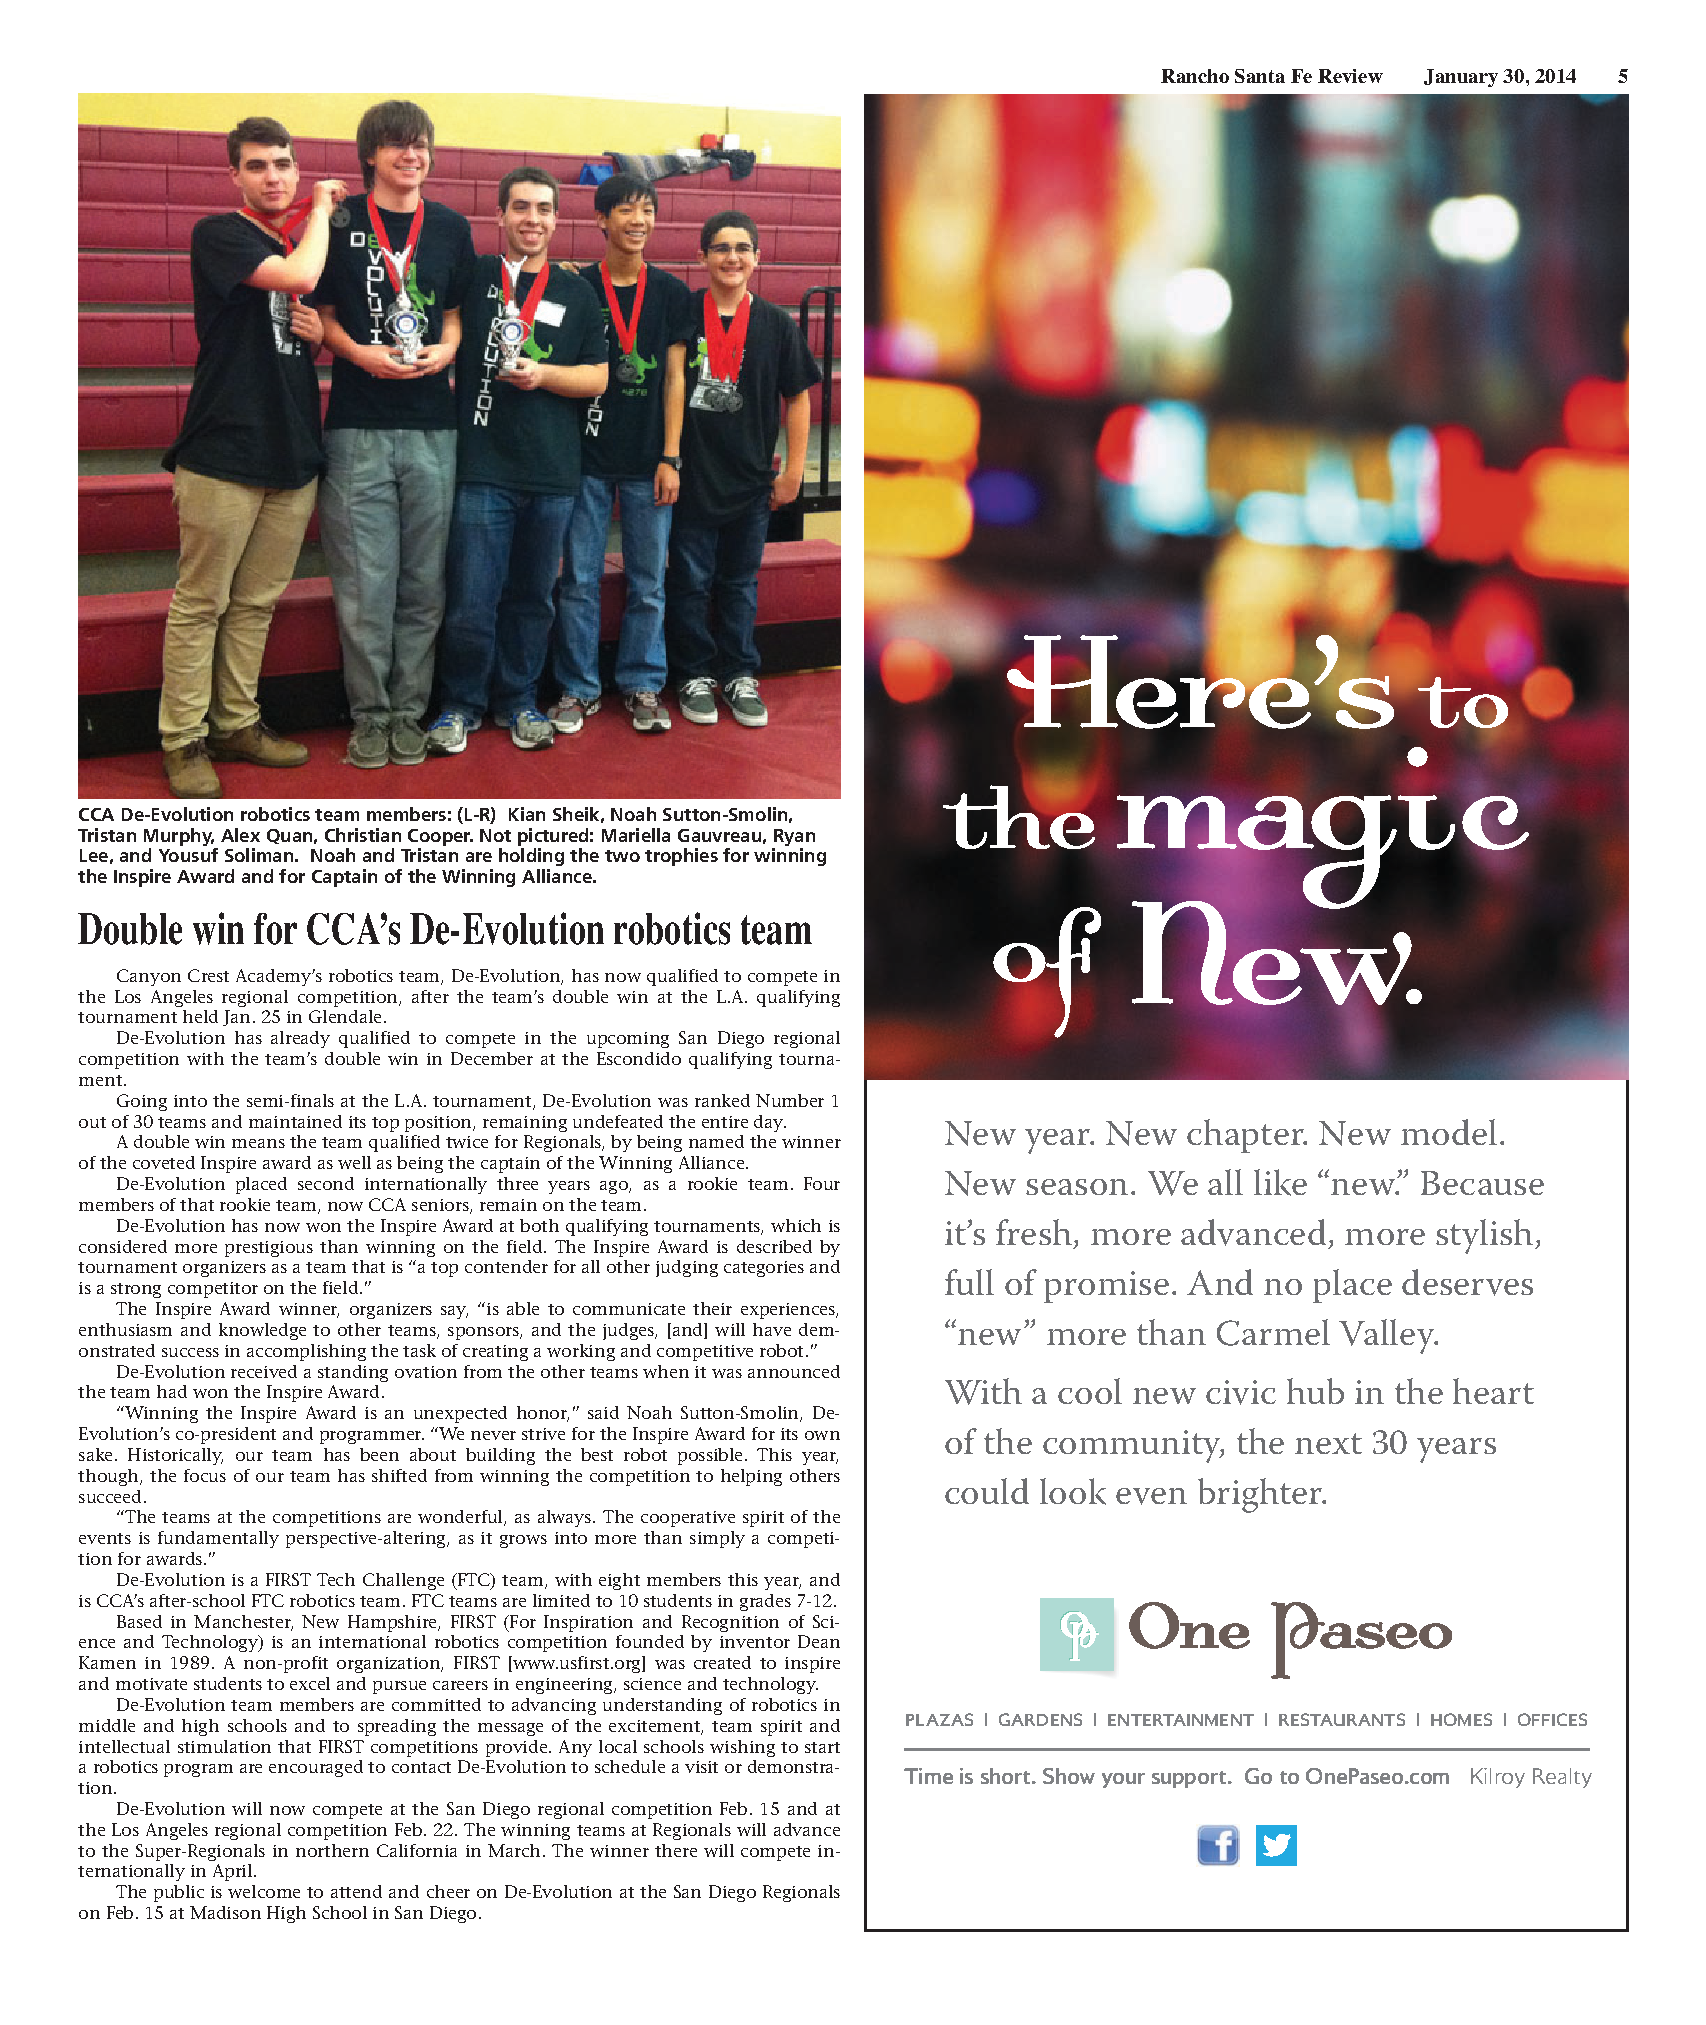
\includepdf[pages={-}]{DoubleWinNewspaper.pdf}
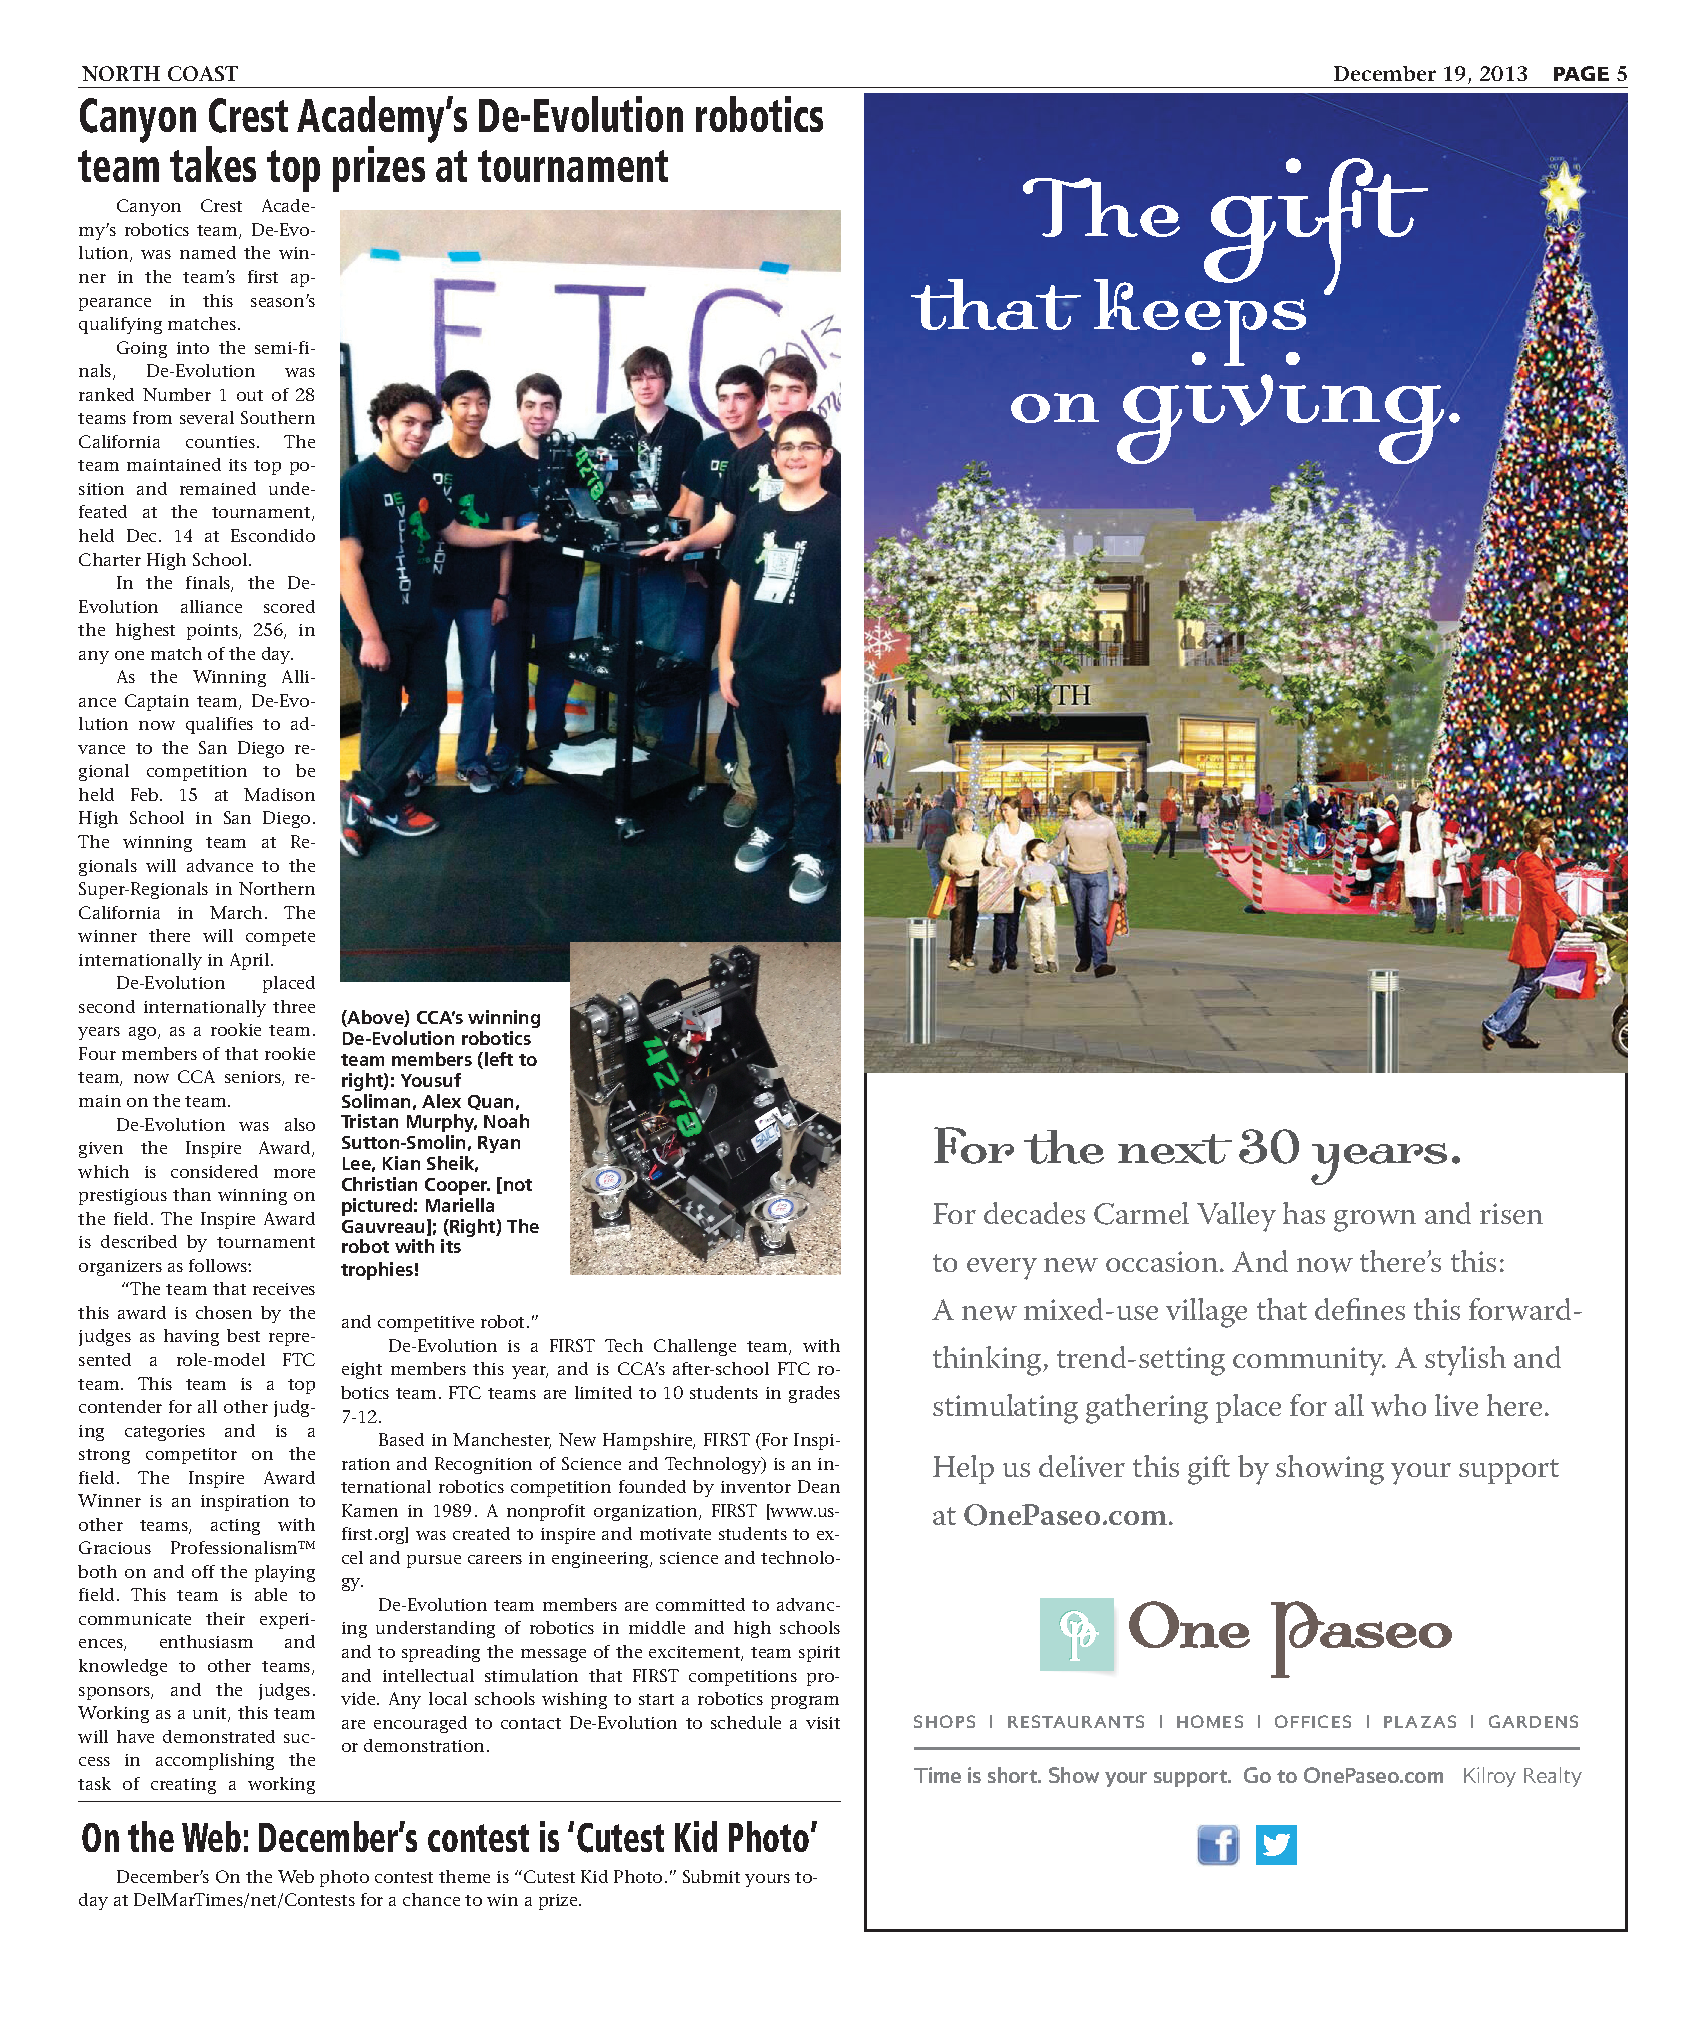
\includepdf[pages={-}]{1219nc-p5.pdf}
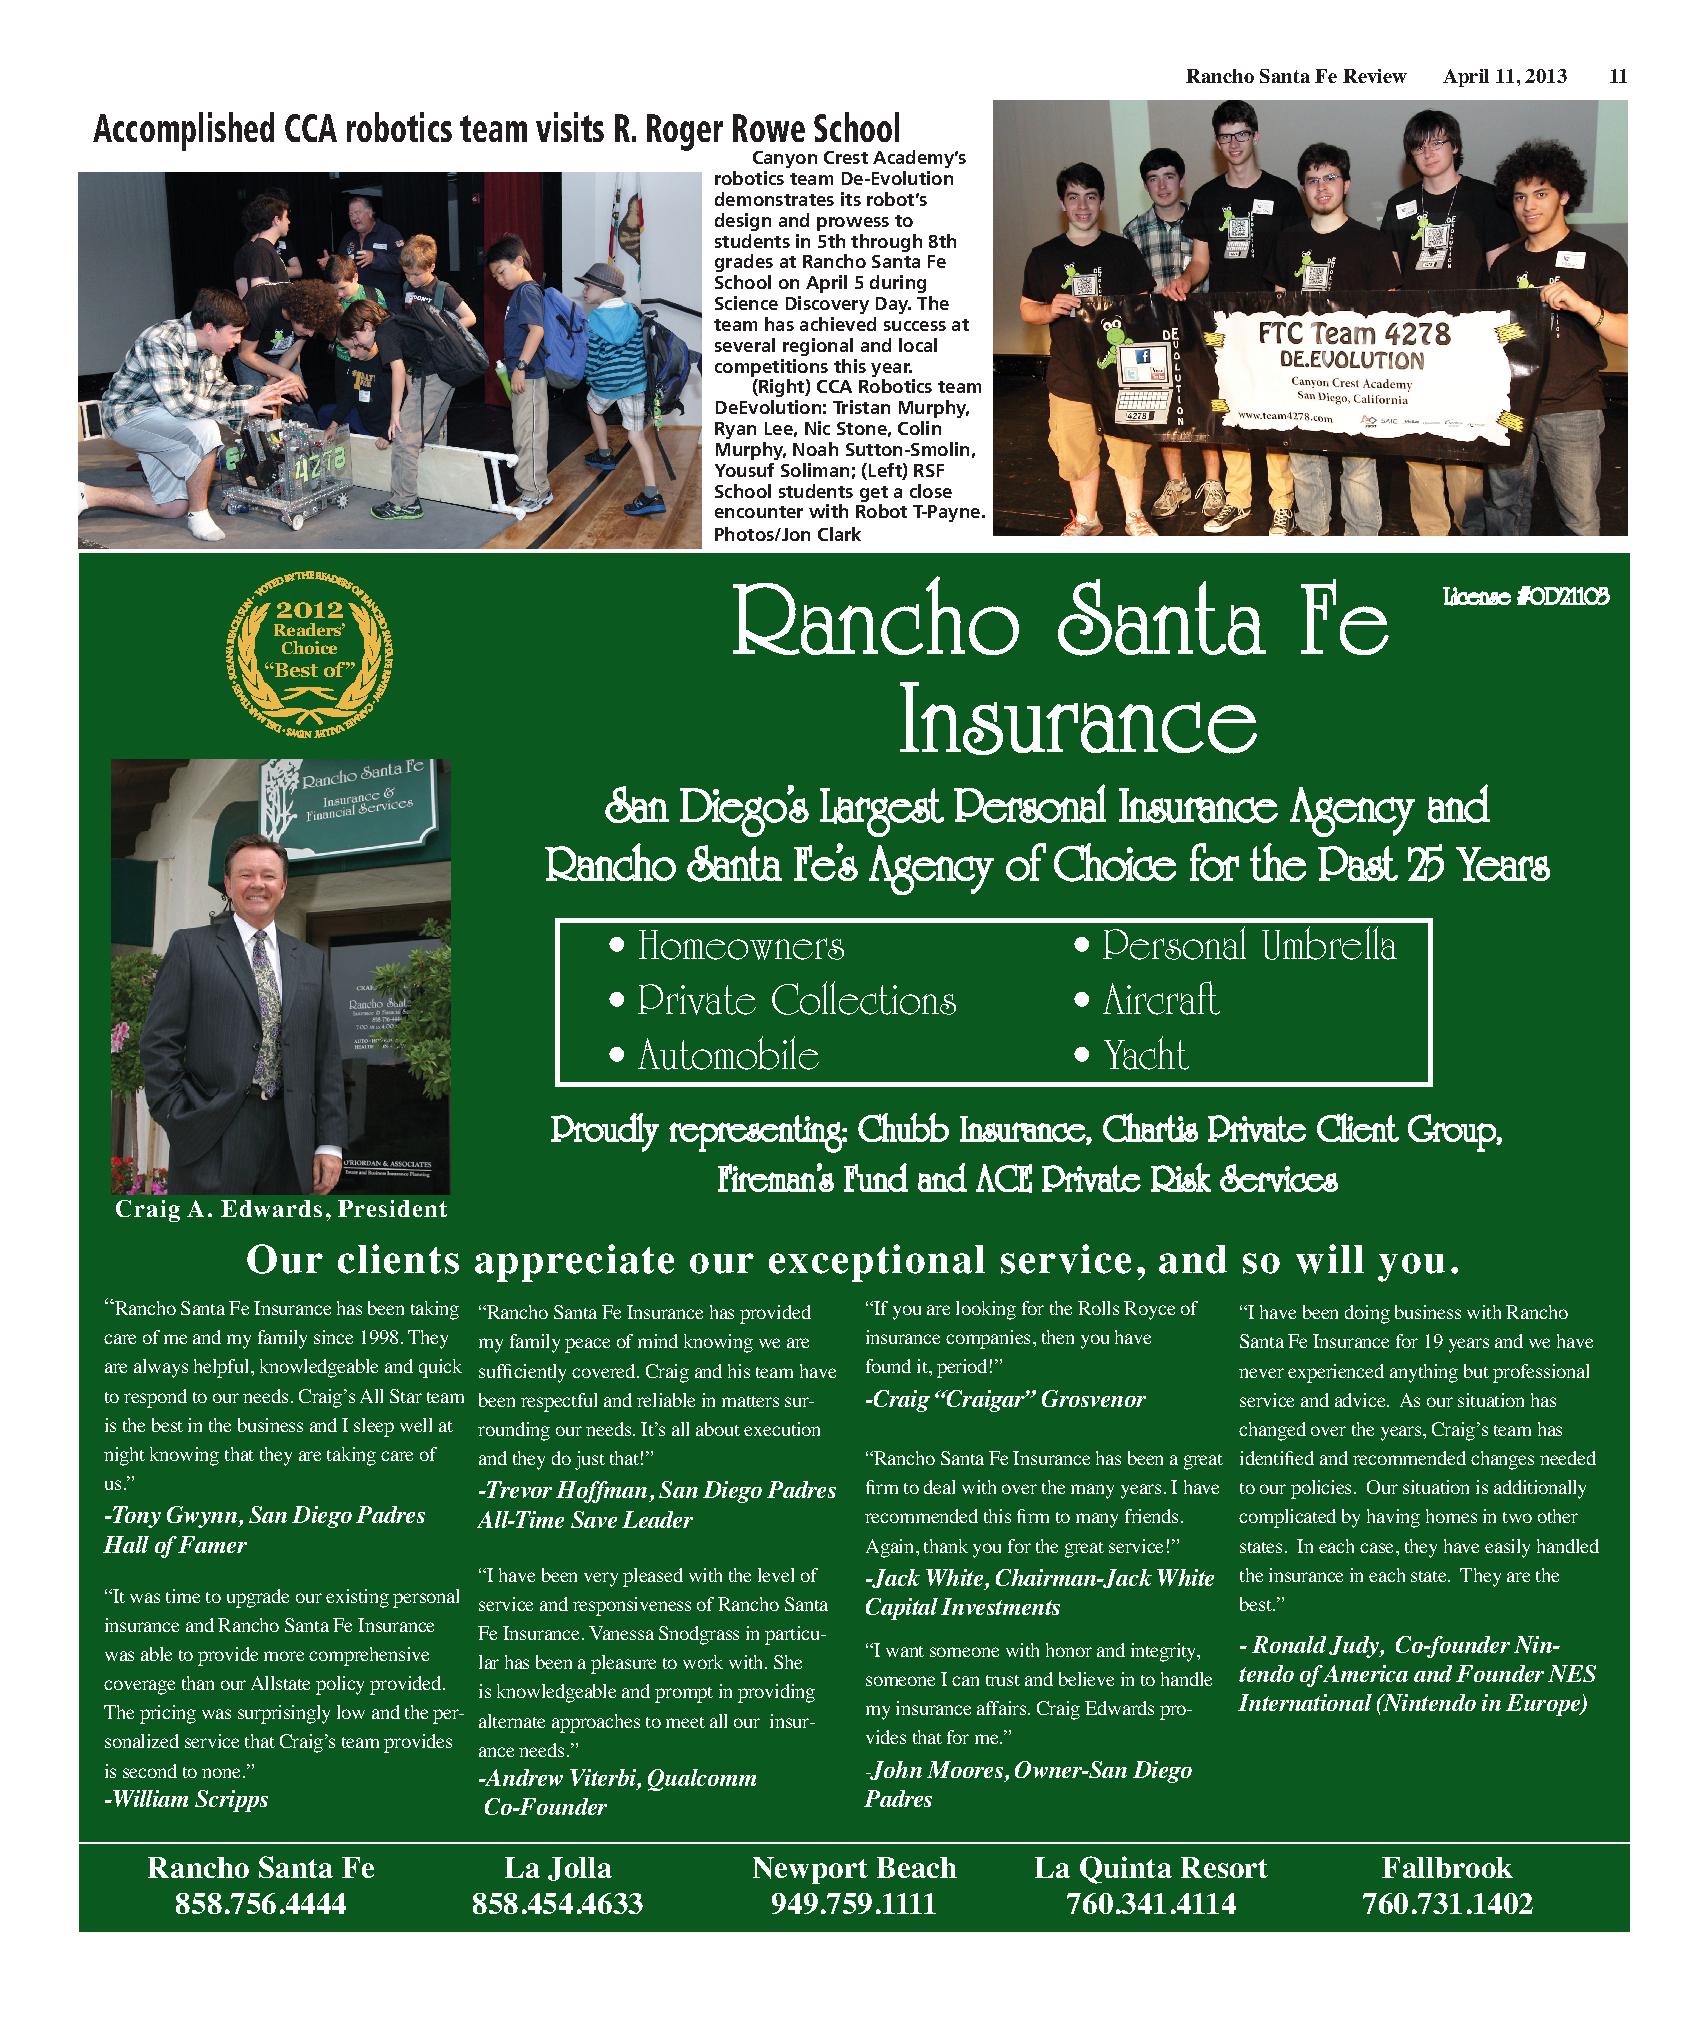
\includepdf[pages={-}]{411rsf-p11.pdf}